\section{Image processing}

\begin{frame}{Datasets} 
	\begin{itemize}
		\item Modified National Institute of Standards and Technology - MNIST (60k/10k)
		\item Canadian Institute For Advanced Research -  CIFAR-10 (50k/10k) and CIFAR-100 (2 level, 500/100) 
		\item Pascal Visual Object Classes (VOC) - 22k images, 20 classes
		\item $\dots$ 
		\item ImageNet 
	\end{itemize}
\end{frame}

\begin{frame}{ImageNet Large Scale Visual Recognition Challenge}

\begin{columns}
	\begin{column}{.5\textwidth}
		\begin{itemize}
			\item Publicly available dataset - ImageNet (14M+, 22k categories)
			\item Annual competition 
			\begin{itemize}
				\item[-] Image classification 
				\item[-] Object detection and localization
			\end{itemize}
			\item Increasing depth 
			\begin{itemize}
				\item[-] 7 layers AlexNet
				\item[-] 19 layers  GoogLeNet
				\item[-] 152 layers ResNet 
			\end{itemize}
 
		\end{itemize}
	\end{column}
	\begin{column}{.5\textwidth}
		\begin{figure}
			\includegraphics[width=1.2\textwidth, center]{figures/ilsvrc_2015_plot}
		\end{figure}
	\end{column}
\end{columns}

 
\end{frame}
\begin{frame}{Using linear layer}
\begin{columns}
	\begin{column}{.7\textwidth}
		\begin{block}{Image as 2D Tensor(Matrix)}
			\begin{center}
			\begin{tabular}{|c|c|c|c|c|}
				\hline
				1 & 2 & 3 & 4 & 5 \\
				\hline
				6 & 7 & 8 & 9 & 10 \\
				\hline
				5 & 4 & 3 & 2 & 1 \\
				\hline
				10 & 9 & 8& 7 & 6 \\
				\hline
			\end{tabular}
			\end{center}
		\end{block}
	\end{column}
	\begin{column}{.3\textwidth}
		\begin{block}{2D $\rightarrow$ 1D}
			\begin{tiny}
				\begin{math}
				\mathbb{W}_{m \times 20} 
				\begin{bmatrix}
				1 \\ 2 \\ 3 \\ 4 \\ 5 \\ 6 \\
				\dots \\
				8 \\ 7\\ 6 \\
				\end{bmatrix} 
				+ \mathbb{B}_{m\times 1}
				\end{math}			
			\end{tiny}
		\end{block}
	\end{column}
\end{columns}
\end{frame}

\begin{frame}{2D Convolution Example}
	\begin{figure}
		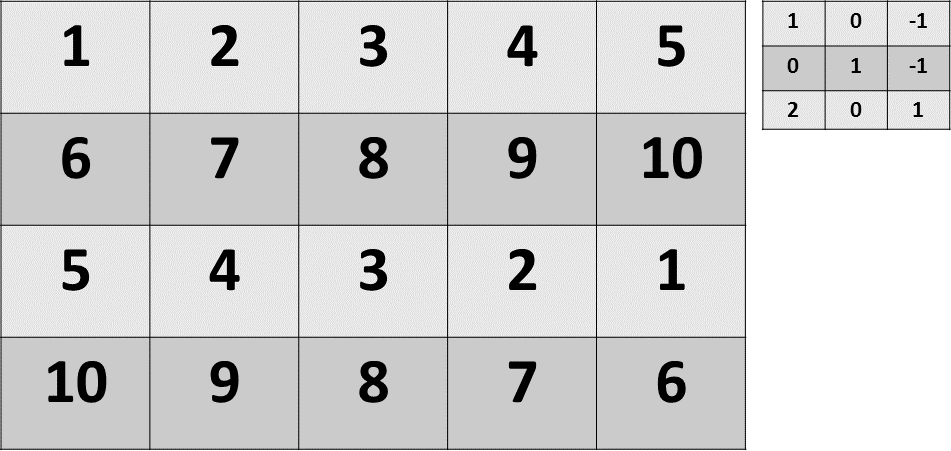
\includegraphics[width=.7\textwidth, center]{figures/conv-slide1-cropped}
	\end{figure}
\end{frame}

\begin{frame}{2D Convolution Example}
	\begin{figure}
		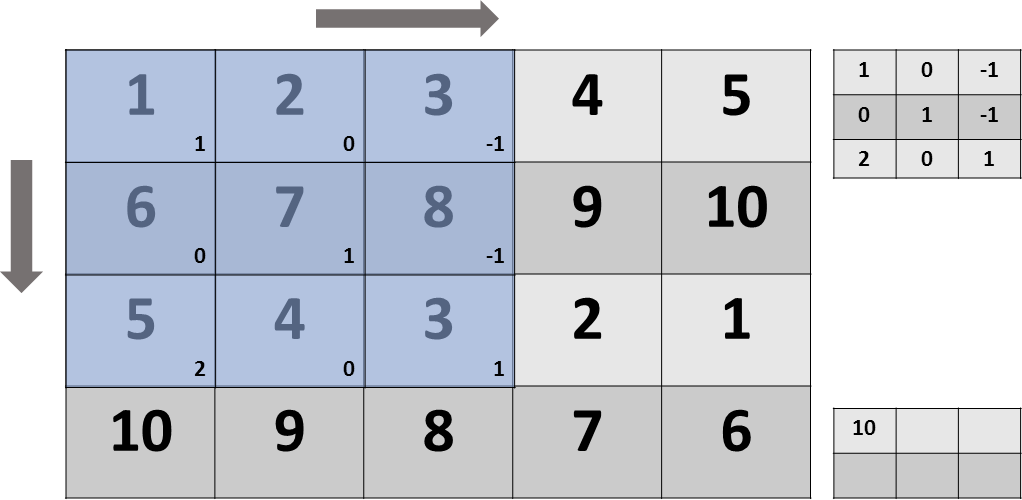
\includegraphics[width=.7\textwidth, center]{figures/conv-slide2-cropped}
	\end{figure}
	\begin{align*}
		(1\times 1)+(2\times 0)+(3\times-1)+ \\
	(6\times 0) + (7 \times 1) + (8 \times -1)+ \\
	(5\times 2) + (4\times 0) + (3\times 1)  
	\end{align*}

\end{frame}

\begin{frame}{2D Convolution Example}
	\begin{figure}
		\includegraphics[width=.7\textwidth, center]{figures/conv-slide3-cropped}
	\end{figure}
\end{frame}

\begin{frame}{2D Convolution Example}
	\begin{figure}
		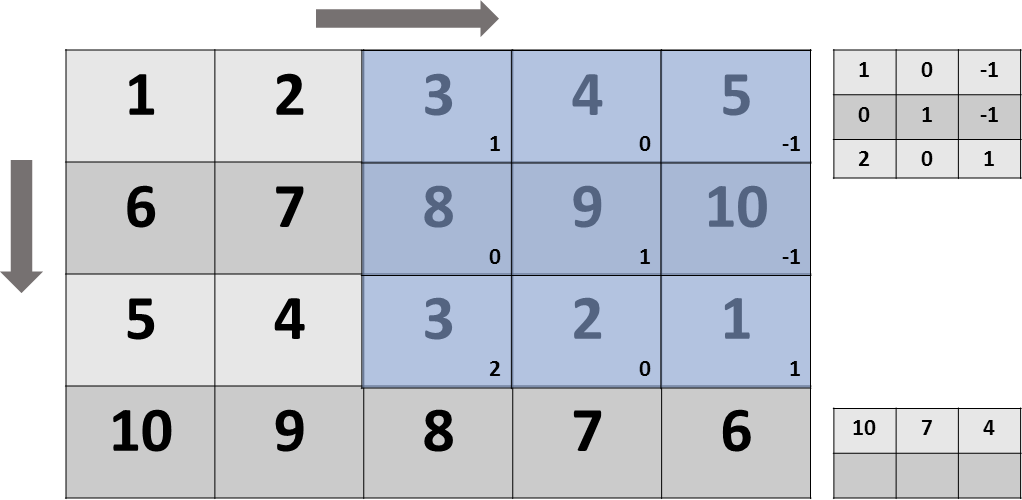
\includegraphics[width=.7\textwidth, center]{figures/conv-slide4-cropped}
	\end{figure}
\end{frame}

\begin{frame}{2D Convolution Example}
	\begin{figure}
		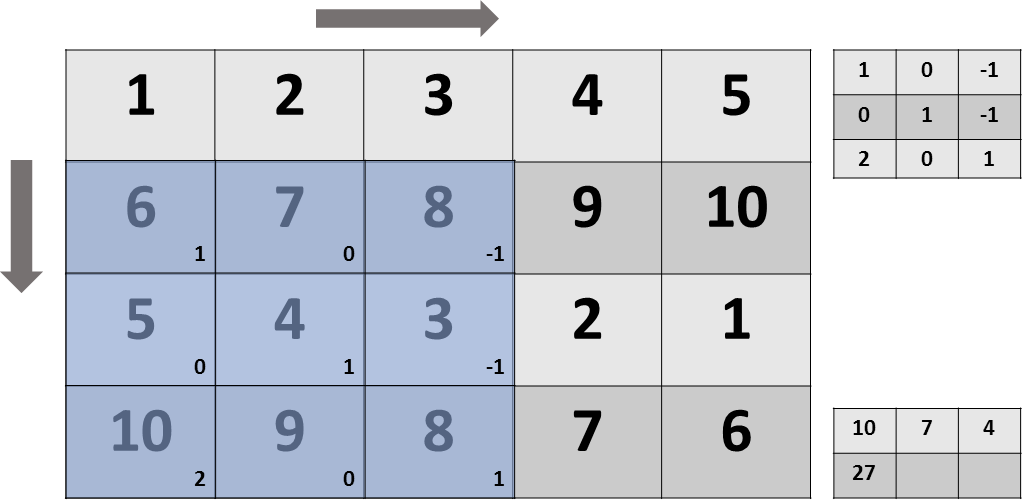
\includegraphics[width=.7\textwidth, center]{figures/conv-slide5-cropped}
	\end{figure}
\end{frame}

\begin{frame}{2D Convolution} 
	\begin{itemize}
		\item Bias 
		\item Stride 
		\item Padding 
		\item Layers or channels 
	\end{itemize}
\end{frame}
\begin{frame}{Pooling}
\end{frame}
